\documentclass[12pt]{article}


%--------- Packages ----------------

\usepackage{graphicx} % Required for inserting images
\usepackage[a4paper,left=1in,right=1in,top=1in,bottom=1in]{geometry}
\usepackage{newtxtext} % If you need to use Time New Roman
\usepackage{newtxmath} % If you need to use Time New Roman
\usepackage[style=apa,backend=biber]{biblatex}
\usepackage[british]{babel}
\usepackage{csquotes}
\usepackage{bookmark}
\usepackage{hyperref}
\usepackage{setspace}
\usepackage{fancyhdr}
\usepackage[font=footnotesize,justification=centering]{caption}
\usepackage{hyperref}
\usepackage{float}
\usepackage{setspace}

%--------- Set Up ------------------
\setstretch{1.5}
\pagestyle{fancy}
\fancypagestyle{plain}{%
  \renewcommand{\headrulewidth}{0pt}%
  \fancyhf{}}
\addbibresource{references.bib}


% --- title insert (check title.tex for more)----------

\title{TITLE} % TITLE HERE 
\author{ Student  \\ Student  \\   Student \\  Student \\ Student \\} % AUTHOR HERE

%-------- Document -----------------

\begin{document}


\begin{titlepage}


\newcommand{\HRule}{\rule{\linewidth}{0.5mm}} % Defines a new command for the horizontal lines, change thickness here

% ----- Logo UM ---------

\center
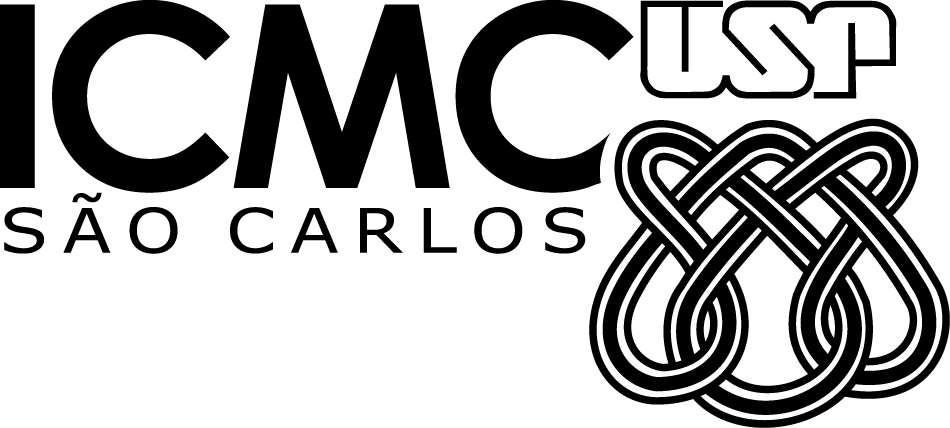
\includegraphics[width=10
cm]{Graphics/LogoICMC.png}\\[1cm]


\textsc{\large Aprendizado de Máquina Aplicado a Problemas}\\[1.5cm]

\makeatletter
\rule{\linewidth}{0.2 mm} \\[0.4 cm]
{\huge\bfseries Educação \par} \
\rule{\linewidth}{0.2 mm} \\[1.0 cm]

\begin{minipage}{0.4\textwidth}
\begin{flushleft} 
\end{flushleft}
\end{minipage}
~
\vspace{1cm}
\vspace{7cm}
\makeatother
{\large 2024}\\[2cm] % Date, change the \today to a set date if you want to be precise
\vfill % Fill the rest of the page with whitespace





\end{titlepage}




\fancyhf{}
\setlength{\headheight}{33pt}
\fancyhead[L]{\nouppercase{\leftmark}}
\fancyhead[R]{
\includegraphics[width=0.7cm]{Graphics/MiniLOGO.png}}
\fancyfoot[R]{ \bf\thepage\ \rm }
\fancyfoot[L]{\emph{Aprendizado de Máquina Aplicado a Problemas} }

\newpage
\tableofcontents
\newpage
\newpage
\section{Introdução}

\par Neste documento, foi feita a análise de correlação entre os atributos de uma base de dados de taxas educacionais e de \textit{IDH}. Para extrair informação do conjunto de dados, os atributos serão segmentados por nível de escolaridade, ou seja, dados do ensino médio, fundamental e infantil serão analisados de forma a se obter uma relação entre os próprios conjuntos e entre os demais atributos, incluindo o atributo alvo.

\subsection{Tratamento de valores faltantes}

\par Dado que existem valores numéricos faltantes de certos atributos na base, faz-se a média aritmética dos valores da mesma coluna dos objetos pertencentes ao mesmo estado. Assim, é feita uma aproximação coerente do valor real para análise.
\section{Resultados}

\subsection{Análise geral do conjunto}

\par Analisando o conjunto de dados de maneira holística na 
Figura \ref{fig:hist-idh} é possível observar a distribuição dos objetos do conjunto de acordo com o IDH municipal.

\begin{figure}[H]
    \centering
    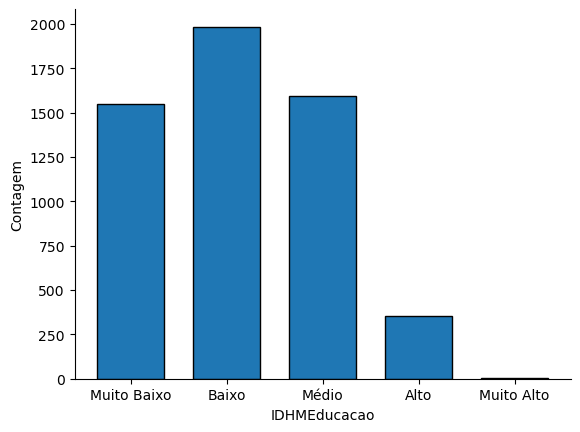
\includegraphics[scale = 0.7]{Graphics/DistribuicaoIDH.png}
    \caption{Histograma dos valores de IDH.}
    \label{fig:hist-idh}
\end{figure}

\par Desse modo, infere-se que há uma concentração significativa de registros nas categorias inferiores do índice, portanto, vê-se que os municípios, em geral, não têm um IDH bom.

\par Para tornar a análise menos complexa, dado que a quantidade de objetos com atributo alvo da classe 'Muito Alto' é da ordem de unidades, os municípios dessa categoria serão integrados à classe 'Alto', sendo analisado conjuntamente.

\subsection{Análise geográfica do IDH dos municípios.}

\par A fim de analisar como o IDH dos municípios de cada região estão distribuídos, faz-se uso do gráfico de barras da Figura \ref{fig:bar-reg}.

\begin{figure}[H]
    \centering
    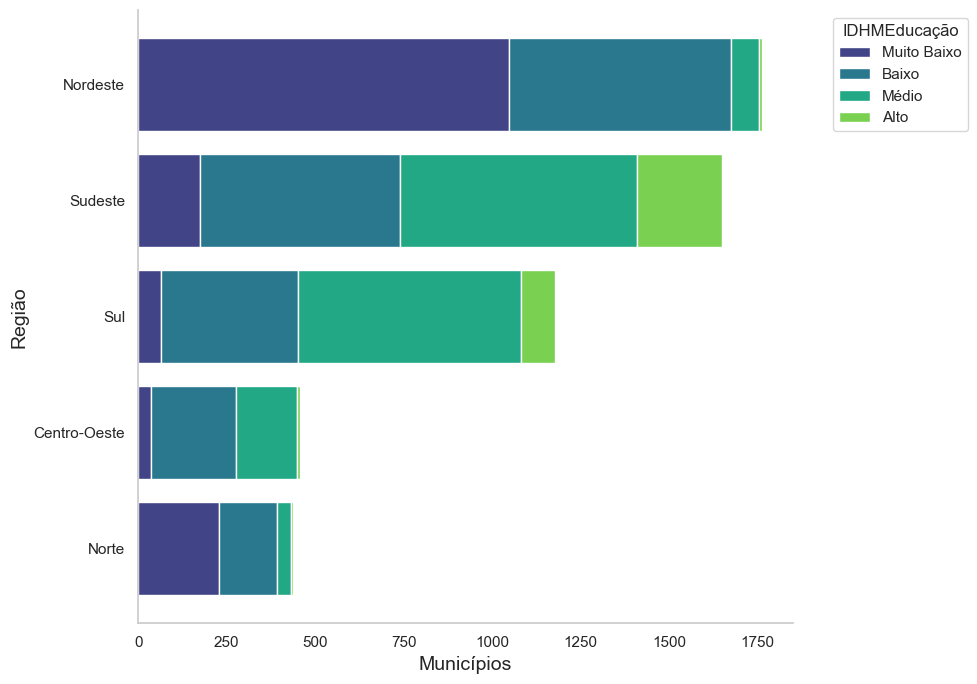
\includegraphics[width=0.75\linewidth]{Graphics/Bars-Regiao.png}
    \caption{Gráfico de barras da quantidade de municípios com a porcentagem de registros pertencentes a cada classe de IDH.}
    \label{fig:bar-reg}
\end{figure}

\par Segundo a ilustração, infere-se que, devido à maior quantidade e à maior proporção de municípios com IDH abaixo da média, os objetos da região Nordeste representam a maior parte dos registros com IDH muito baixo ou baixo. Assim, possíveis políticas públicas podem ser mais efetivas caso aplicadas com enfoque nesses municípios.

\par Ademais, vê-se que a maior parte dos municípios com IDH na média ou acima são das regiões Sul e Sudeste, fator que pode estar relacionado ao elevados índice educacionais das regiões. Além disso, observa-se que as regiões Centro-Oeste e Norte apresentam mais da metade dos municípios com IDH abaixo da média, o que exige uma dose de atenção por parte do estado e da comunidade para amenizar tais indicadores.

\par Posteriormente, para analisar a representação relativa de cada região nas categorias do atributo alvo, utiliza-se o gráfico de barras da Figura \ref{fig:bar-idh}.

\begin{figure}[H]
    \centering
    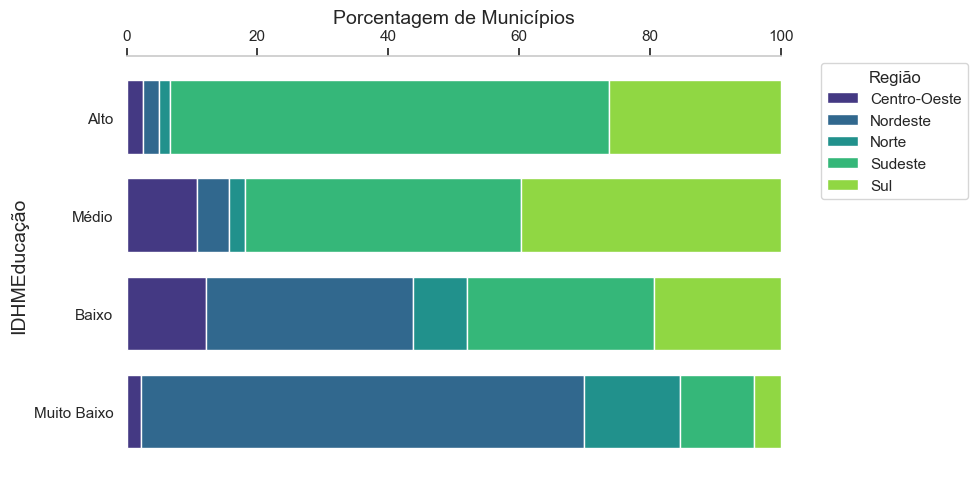
\includegraphics[width=0.75\linewidth]{Graphics/Bars-IDH.png}
    \caption{Gráfico de barras de participação relativa das regiões nas categorias de IDH.}
    \label{fig:bar-idh}
\end{figure}

\par Com base na figura, reitera-se a análise de que grande parte da quota de municípios com IDH na média ou acima pertence às regiões Sul e Sudeste e que os objetos com indicador abaixo da média é do Nordeste, com significante parcela da região Centro-Oeste nas categorias 'Baixo' e 'Médio' e com participação considerável de registros da região Norte entre os indicadores alvo mais baixos.

\subsection{Análise relacional entre os atributos preditivos.}

\subsubsection{Mapas de calor.}
\label{heat-sec}

\par Primeiramente, a fim de analisar a correlação dos atributos numéricos, lança-se mão da tabela de correlação, analisada com dois métodos distintos, com coeficiente de Pearson e de Kendall, e do mapa de calor correspondente, disponibilizados nas Figuras \ref{fig:heat-pear} e \ref{fig:heat-kend}.

\par O atributo alvo foi transformado em uma ordem numérica de 1 a 5, de 'Muito Baixo' para 'Alto' para que a correlação entre a coluna e o restante das variáveis pudesse ser calculada.

\begin{figure}
    \centering
    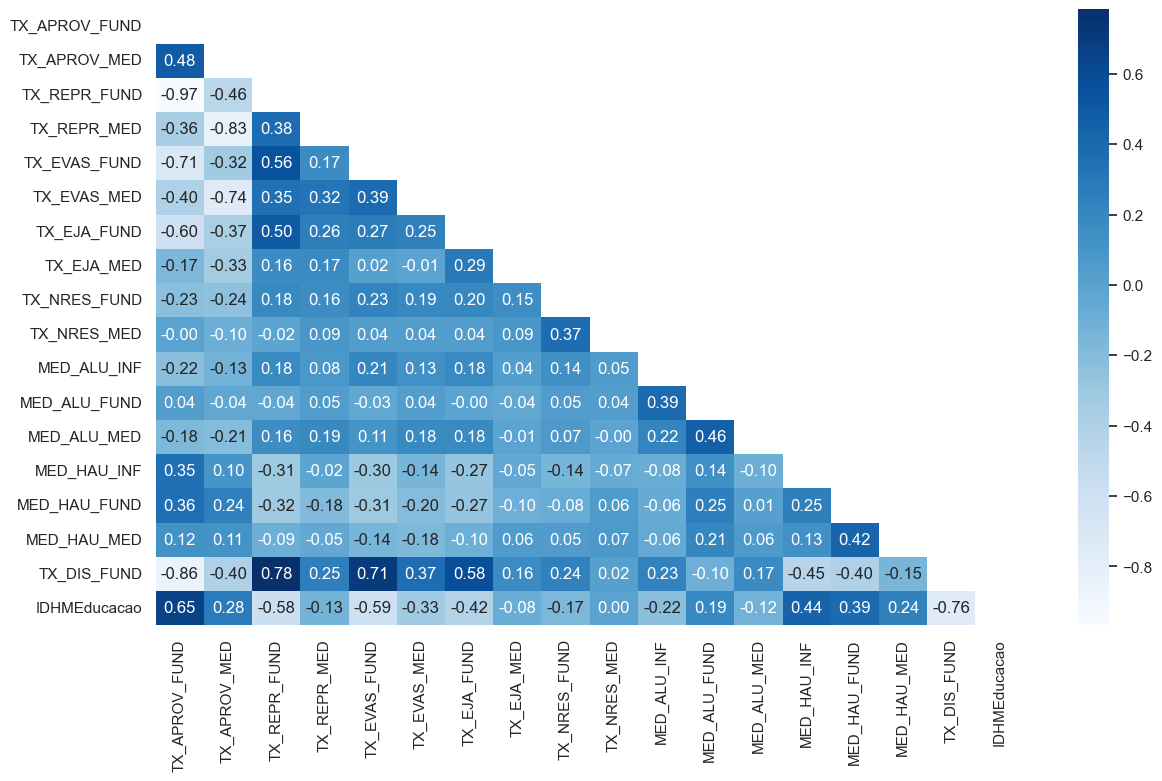
\includegraphics[width=1\linewidth]{Graphics/HeatMapPearson.png}
    \caption{Mapas de calor das correlações de Pearson dos atributos.}
    \label{fig:heat-pear}
\end{figure}

\par A partir da imagem da correlação de Pearson, é possível inferir que o atributo alvo tem alta dependência com a taxa de disfunção idade-série e com as taxas referentes ao ensino fundamental, como aprovação, reprovação e evasão, fator que evidencia uma alta relação desses fatores com o IDH e suas importâncias. Além disso, em relação à taxa de disfunção idade-série, vê-se uma relação consideravelmente alta com as taxas do ensino fundamental.

\begin{figure}
    \centering
    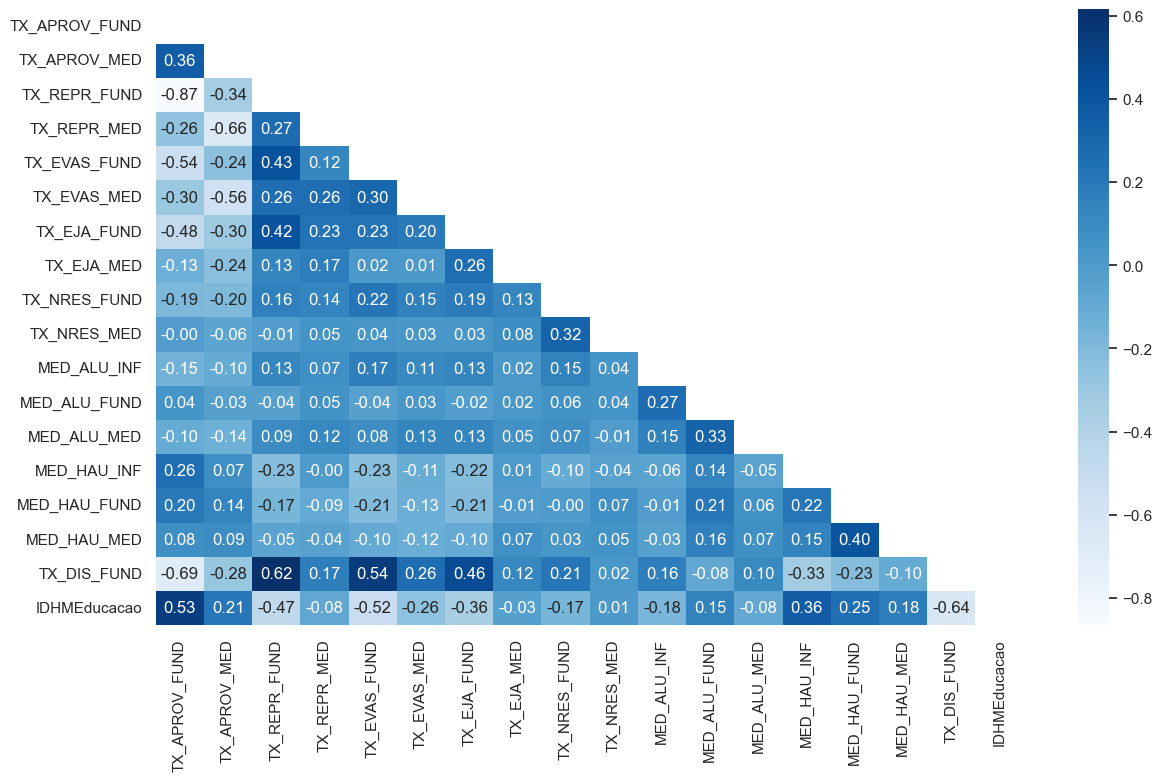
\includegraphics[width=1\linewidth]{Graphics/HeatMapKendall.png}
    \caption{Mapas de calor das correlações de Kendall dos atributos.}
    \label{fig:heat-kend}
\end{figure}

\par Consonante à correlação com coeficiente de Kendall, é possível observar relações análogas à análise de Pearson, reiterando as dependências entre os atributos do conjunto de dados.

\subsubsection{Gráficos de dispersão}

\par Primeiramente, observa-se os mapas de dispersão das taxas referentes ao ensino médio e ao ensino fundamental nas Figuras \ref{fig:fundamental} e \ref{fig:medio}.
 
\begin{figure}[H]
    \centering
    \begin{minipage}{0.45\textwidth}
        \centering
        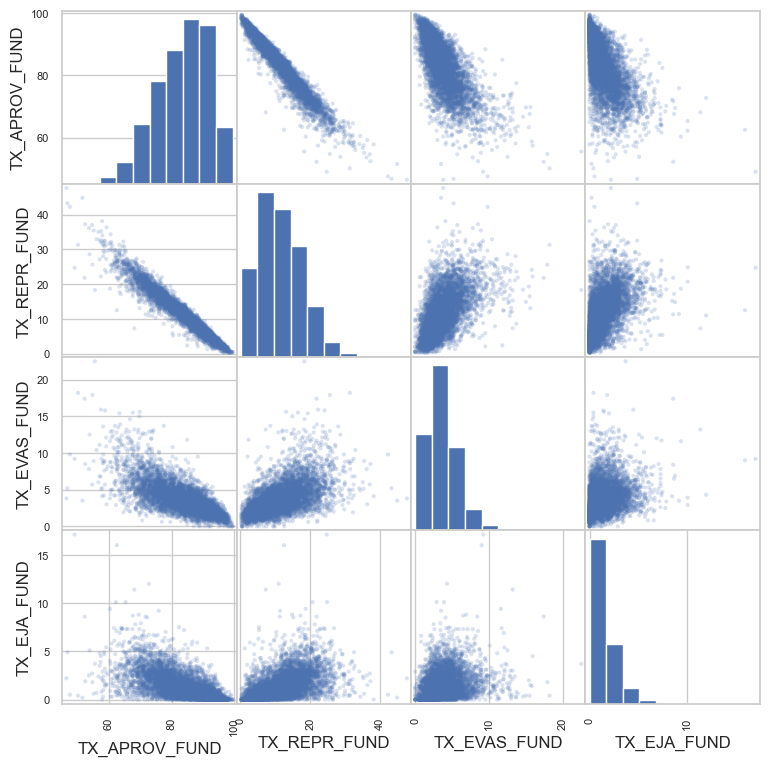
\includegraphics[scale=0.35]{Graphics/ScatterFundamental.png}
        \caption{Gráficos de dispersão e histogramas das taxas do ensino fundamental.}
        \label{fig:fundamental}
    \end{minipage}\hfill
    \begin{minipage}{0.45\textwidth}
        \centering
        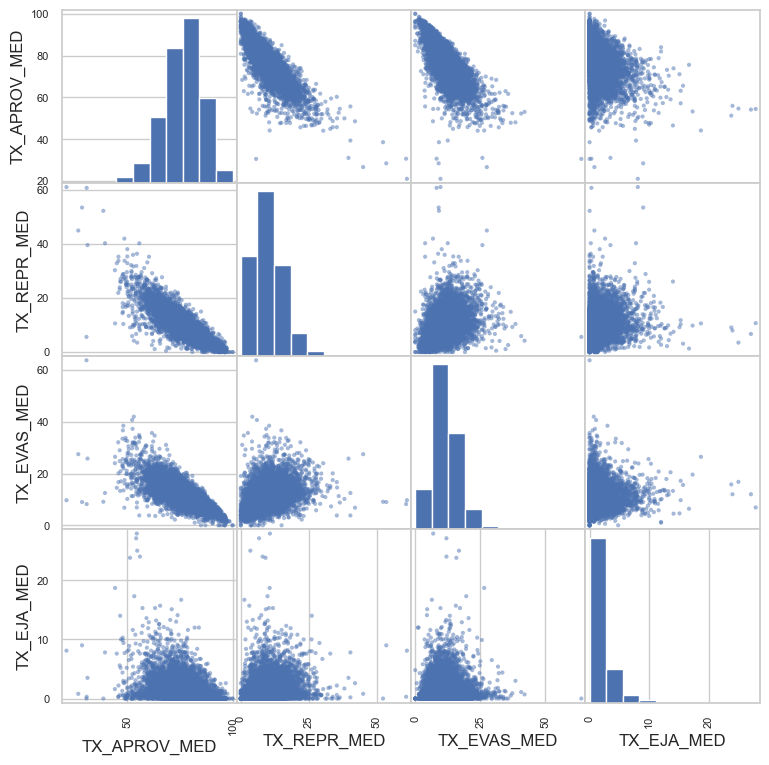
\includegraphics[scale=0.35]{Graphics/ScatterMedio.png}
        \caption{Gráficos de dispersão e histogramas das taxas do ensino médio.}
        \label{fig:medio}
    \end{minipage}
\end{figure}

\par Ao se considerar os mapas de dispersão dos atributos dos níveis de ensino fundamental e médio, infere-se que, principalmente entre os atributos do ensino médio, verifica-se uma fraca correlação linear entre os atributos enquanto os atributos do ensino fundamental se mostram ligeiramente mais relacionados, principalmente nos atributos de taxa de promoção e de repetência. Assim, além dos dois primeiros atributos, conclui-se que os atributos de cada nível não estão fortemente correlacionados entre si.

\par Subsequentemente, a fim de se verificar a relação entre os atributos dos níveis médio e fundamental com a taxa de distorção respectivas, lança-se mão das Figuras \ref{fig:disp-fund} e \ref{fig:disp-med}.

\begin{figure}[H]
    \centering
    \includegraphics[scale = 0.28]{Graphics/DispersãoFundamental.png}
    \caption{Relação das taxas do ensino fundamental da base de dados com a taxa de distorção idade-série no ensino fundamental.}
    \label{fig:disp-fund}
\end{figure}

\par Assim, vê-se que o ensino fundamental demonstrou relação mais forte das taxas com a distorção.

\begin{figure}[H]
    \centering
    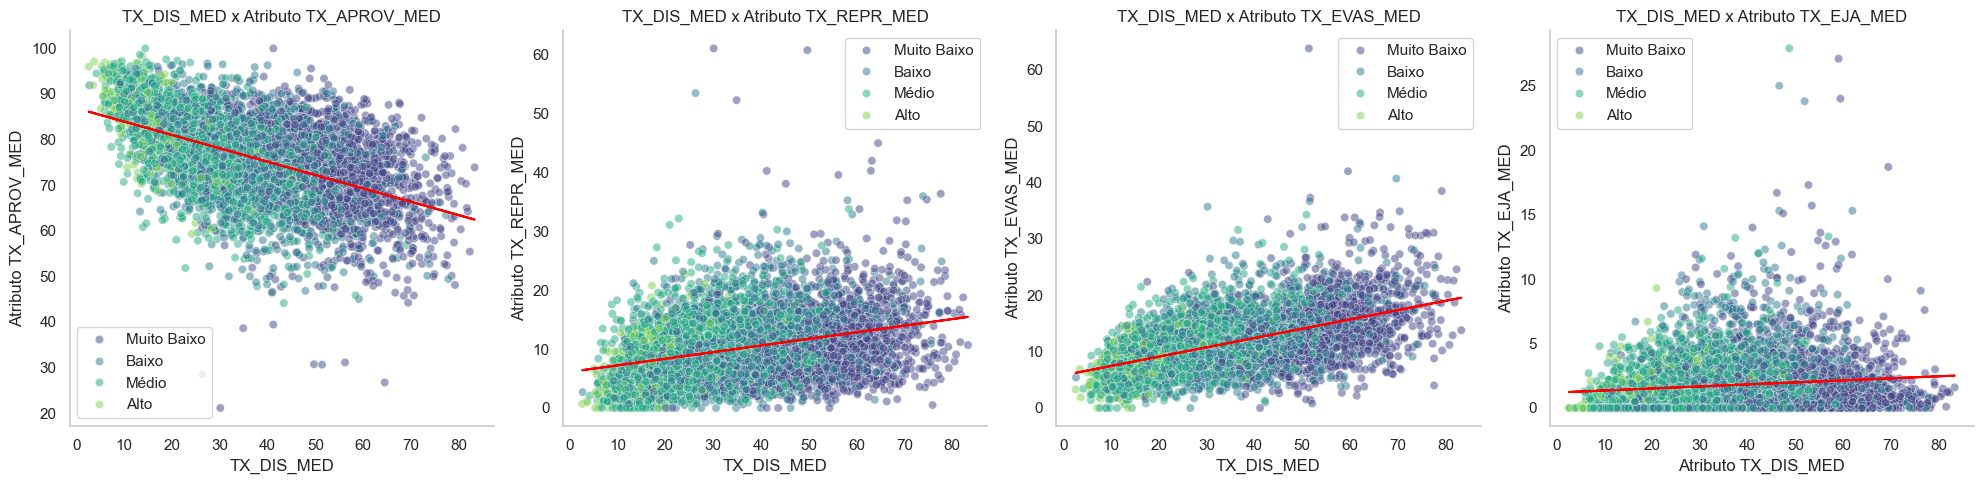
\includegraphics[scale = 0.28]{Graphics/Dispersão médio.png}
    \caption{Relação das taxas do ensino médio da base de dados com a taxa de distorção idade-série no ensino médio.}
    \label{fig:disp-med}
\end{figure}

\par A fim de se verificar a hipótese de que a média de alunos e de aula-hora no ensino infantil impacta as etapas posteriores de educação, verifica-se os mapas de dispersão em função das taxas de distorção de idade nas Figuras \ref{fig:disp-inf-fund} e \ref{fig:dis-inf-med}.

\begin{figure}[H]
    \centering
    \begin{minipage}{0.45\textwidth}
        \centering
        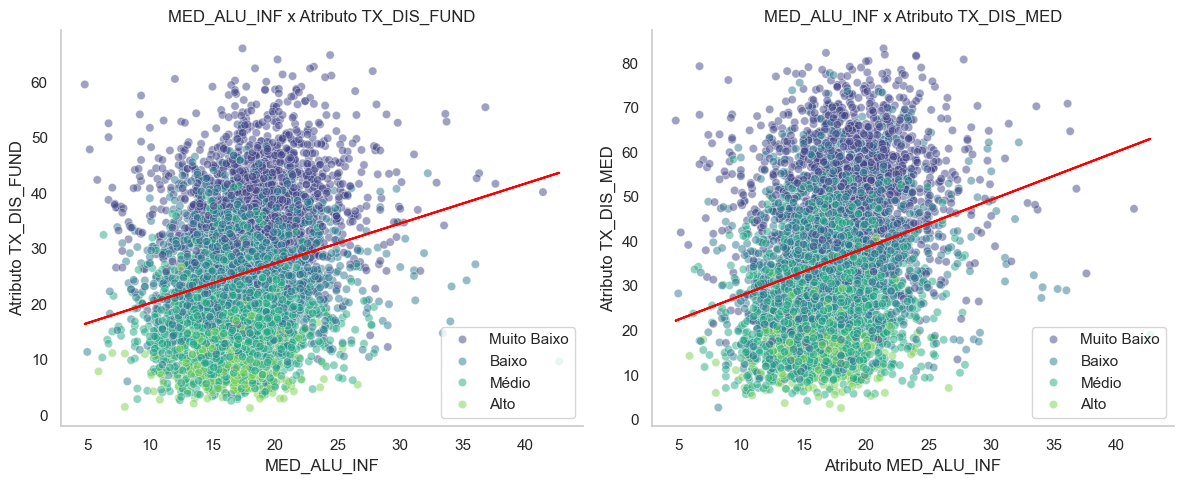
\includegraphics[scale=0.25]{Graphics/DispersaoInfantilAlunosDistorcao.png}
        \caption{Relação entre a média de alunos no ensino infantil com a distorção idade-série no ensino fundamental.}
        \label{fig:disp-inf-fund}
    \end{minipage}\hfill
    \begin{minipage}{0.45\textwidth}
        \centering
        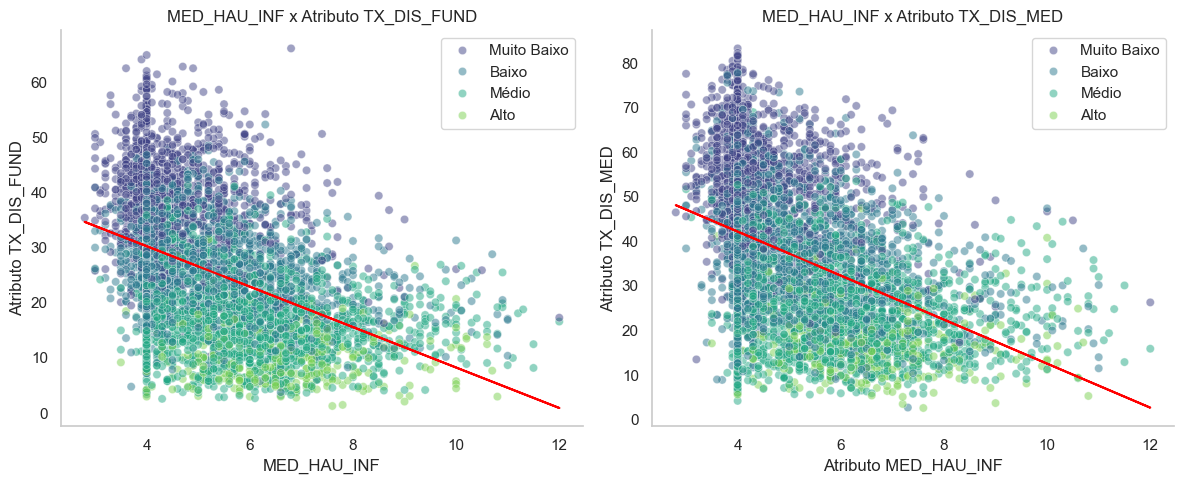
\includegraphics[scale=0.25]{Graphics/DispersaoInfantilHorasDistorcao.png}
        \caption{Relação entre a média de horas-aula no ensino infantil com a distorção idade-série no ensino fundamental..}
        \label{fig:dis-inf-med}
    \end{minipage}
\end{figure}

\par Após a visualização, é razoável concluir que a relação é fraca pelo comportamento pouco compátivel com a linearidade, demonstrando, assim, pouca proporção causa-consequência dos atributos.

\subsection{Análise relacional entre os atributos preditores e o atributo alvo.}

\subsubsection{Boxplots.}

\par A priori, com intuito de verificar a correlação do atributo alvo com as quatro taxas iniciais de cada nível de ensino, faz-se uso do \textit{boxplot} nas Figuras \ref{fig:box-fund} e \ref{fig:box-med}.

\begin{figure}[H]
    \centering
    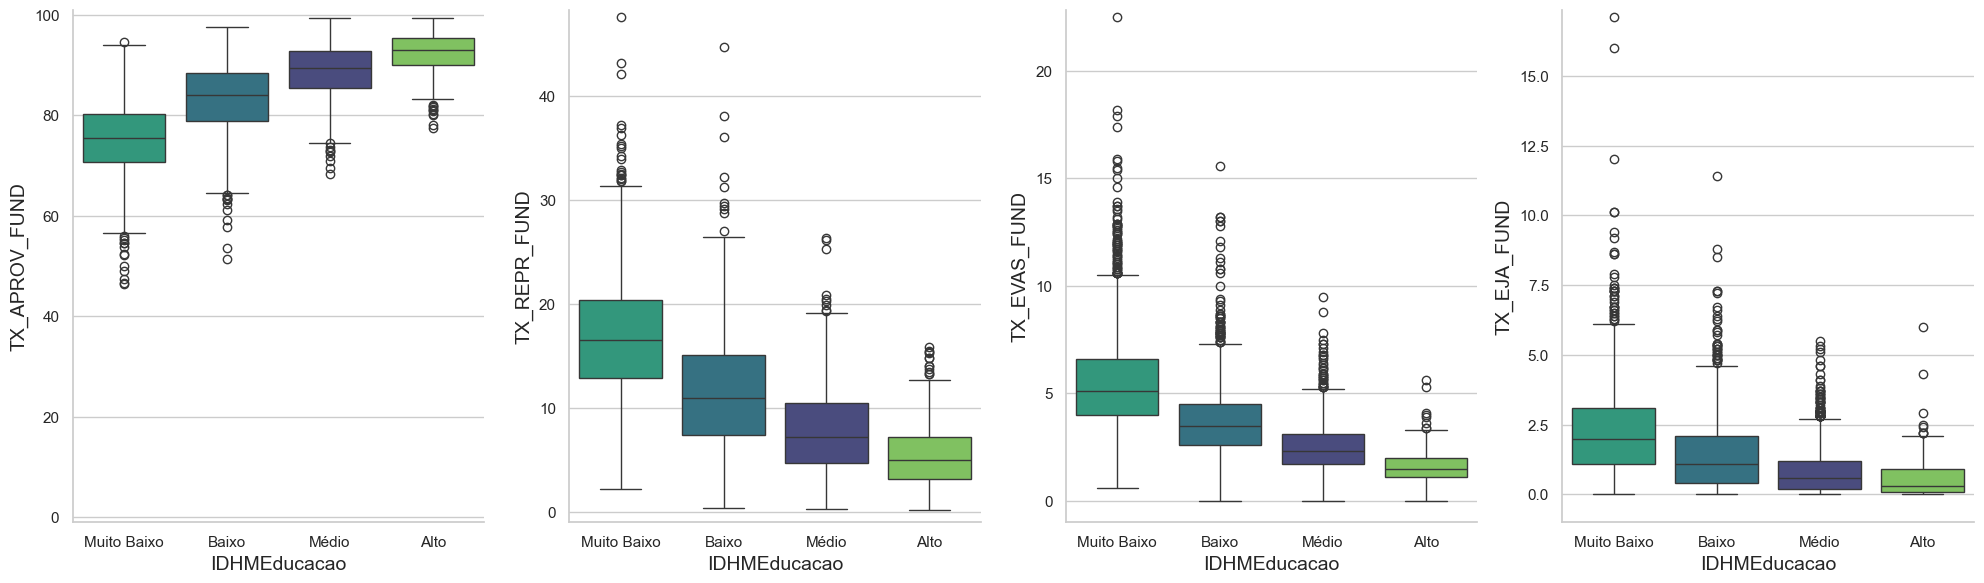
\includegraphics[scale = 0.3]{Graphics/BoxFundamentalIDH.png}
    \caption{Boxplots das taxas relacionadas ao ensino fundamental em cada categoria de IDH.}
    \label{fig:box-fund}
\end{figure}

\begin{figure}[H]
    \centering
    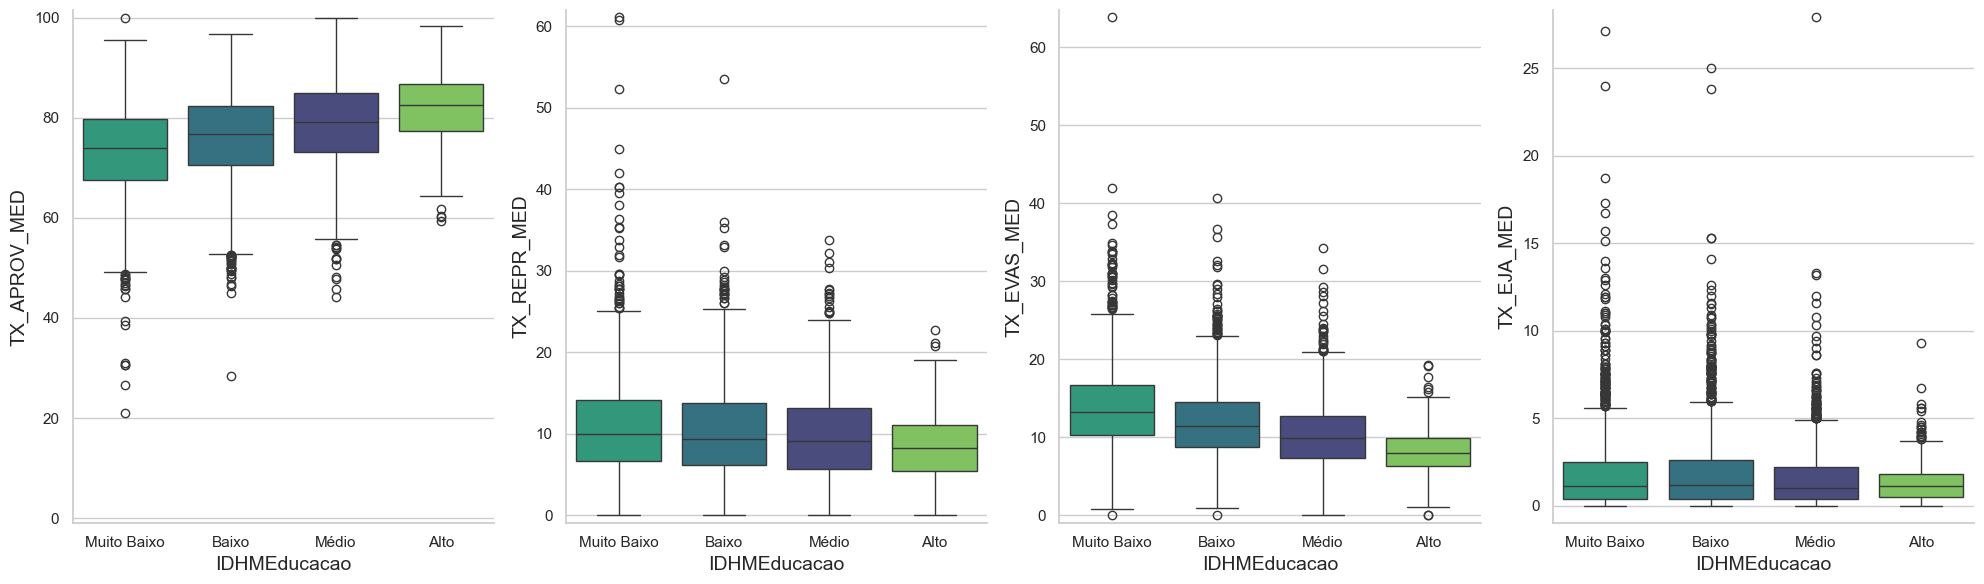
\includegraphics[scale = 0.3]{Graphics/BoxMedioIDH.png}
    \caption{Boxplots das taxas relacionadas ao ensino médio em cada categoria de IDH.}
    \label{fig:box-med}
\end{figure}

\par Após visualização, infere-se que o \textit{IDH} de um município tem relação mais próxima com as taxas do ensino fundamental em comparação ao ensino médio graças à maior proporcionalidade entre os atributos e menos inconsistência, o que legitima o mapa de calor abordado no tópico \ref{heat-sec}.

\par Após, a fim de se verificar a relação das médias de alunos e de horas-aula, Figuras \ref{fig:disp-malu} e \ref{fig:disp-mhau}, respectivamente, e do atributo alvo, vê-se que ambos não apresentam relação forte com o \textit{IDH}, porém, é razoável concluir que a média de horas-aula é mais relevante para o \textit{IDH} em comparação à média de alunos por turma nos três níveis de ensino, sendo negativo em relação á média de alunos, exceto no ensino fundamental, e positiva em relação às horas-aula.

\begin{figure}[H]
    \centering
    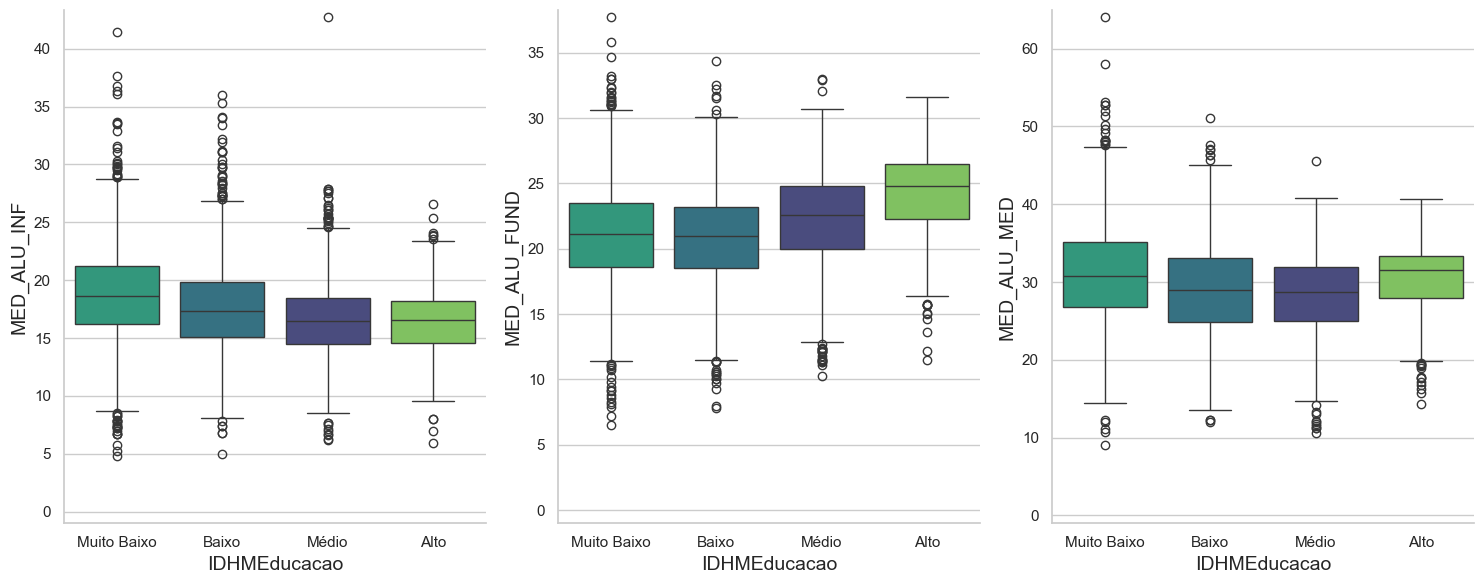
\includegraphics[scale = 0.3]{Graphics/BoxAlunosIDH.png}
    \caption{Boxplots da média de alunos por turma em relação a cada categoria de IDH.}
    \label{fig:disp-malu}
\end{figure}

\begin{figure}[H]
    \centering
    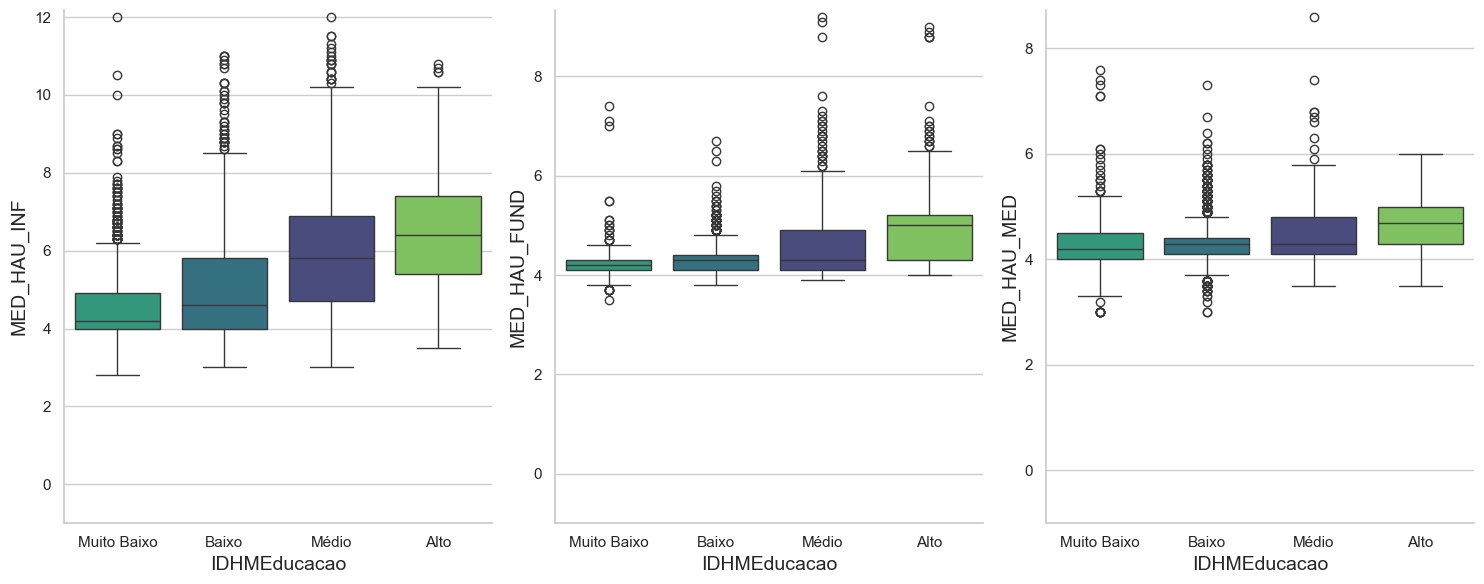
\includegraphics[scale = 0.3]{Graphics/BoxHorasIDH.png}
    \caption{Boxplots da média de horas-aula em relação a cada categoria de IDH.}
    \label{fig:disp-mhau}
\end{figure}

\par Por fim, verifica-se a relação entre a taxa de distorção idade-série e o \textit{IDH} do município na Figura \ref{fig:disp-dis}.

\begin{figure}[H]
    \centering
    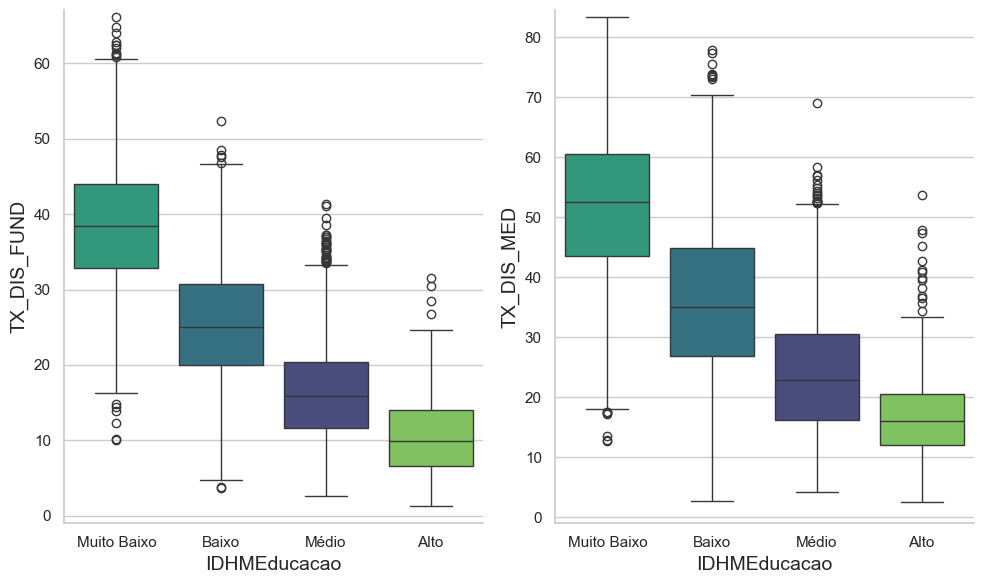
\includegraphics[scale = 0.3]{Graphics/BocDistorcaoIDH.png}
    \caption{Boxplots das taxas de distorção idade-série em relação a cada categoria de IDH.}
    \label{fig:disp-dis}
\end{figure}

Assim, confirmando o fato representado nos mapas de calor no tópico \ref{heat-sec}, infere-se que ambas as taxas de distorção idade-série, tanto no ensino fundamental, quanto no ensino médio, tem forte correlação negativa com o atributo alvo.
\section{Conclusão}

\par Portanto, foi possível inferir que, em um conjunto de dados desbalanceado, em que as classes com \textit{IDH} menor tem número significativamente superior de representantes. 

\par Em relação à análise geográfica, observa-se que a região Nordeste se evidencia como a mais carente em função do atributo, seguida das regões Norte e Centro-Oeste. Opostamente, as regiões Sudeste e Sul apresentaram uma proporção maior de municípios com IDH médio ou acima.

\par Na questão das correlações dos atributos preditivos, percebe-se que as quatro taxas iniciais dos dois níveis de ensino, as quais não são fortemente correlacionadas entre si, são relevantes para a taxa de distorção idade-série, a qual se configurou como atributo preditivo fortemente relacionado ao atributo alvo, além de que, as taxas que tangem à educação infantil não apresentaram tanta relevância para estimar a taxa de distorção idade-série. Além disso, nos boxplots, foi possível concluir que as taxas do par de níveis escolares, fundamental e médio, são ambas significantes para estimar a categoria de \textit{IDH} de um município, dando ênfase às taxas do ensino fundamental. Ademais, as médias de alunos e de horas-aula demonstraram ligeira relevância de predição em comparação às taxas de promoção, repetência, evasão e migração, porém a média de horas-aula possui relação mais próxima à linearidade. Além disso, viu-se que as taxas de distorção idade-série tem elevada correlação com o atributo alvo. Por fim, é razoável enfatizar que as relações ilustradas no mapa de calor foram legitimadas.

\printbibliography
\pagebreak
\newpage
\end{document}
